\documentclass[varwidth]{standalone}

\usepackage{amsmath}
\usepackage[dvipsnames]{xcolor}
\usepackage{tikz}
\usetikzlibrary{arrows.meta}
\usetikzlibrary{backgrounds}
\usetikzlibrary{calc}
\usetikzlibrary{fit}
\usetikzlibrary{positioning}
\usetikzlibrary{patterns}
\usetikzlibrary{shapes}
\usetikzlibrary{shapes.misc}


\begin{document}
\resizebox{\textwidth}{!}{%
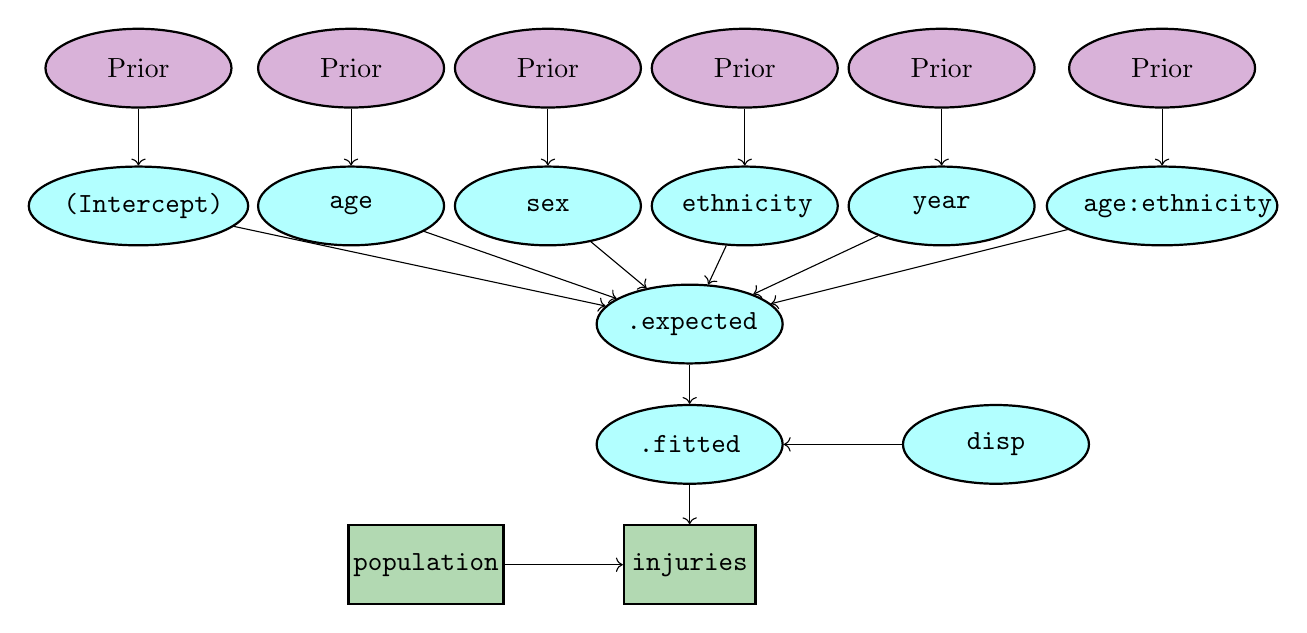
\begin{tikzpicture}
  [
    node distance = 1.5cm and 1.5cm,
    node/.style = {thick, draw, text width = 1.6cm,
                  minimum height = 1cm, align = center, inner sep = 1pt},
    obs/.style = {node, rectangle, text width = 1.6cm, fill=Green!30},
    unobs/.style = {node, ellipse, fill=Cyan!30},
    prior/.style = {unobs, fill=Purple!30},
    arrow/.style  = {> = stealth, thick, length=8pt},
  ]

  \node[obs] (y) {\texttt{injuries}};
  \node[obs, text width = 1.9cm] [left = of y] (w) {\texttt{population}}
  edge[->](y);

  \node[unobs][above = of y, yshift = -1cm] (gamma) {\texttt{.fitted}}
    edge[->](y);

      \node[unobs][above = of gamma, yshift = -1cm] (mu) {\texttt{.expected}}
    edge[->](gamma);

      \node[unobs][right = of gamma] (disp) {\texttt{disp}}
    edge[->](gamma);

    \node[unobs, text width = 1.9cm] [above of = mu, xshift = -7cm, yshift = 0cm] (beta_int) {\texttt{(Intercept)}}
      edge[->](mu);
    \node[unobs] [right of = beta_int, xshift = 1.2cm] (beta_age) {\texttt{age}}
      edge[->](mu);
    \node[unobs] [right of = beta_age, xshift = 1cm] (beta_sex) {\texttt{sex}}
      edge[->](mu);
    \node[unobs] [right of = beta_sex, xshift = 1cm] (beta_eth) {\texttt{ethnicity}}
      edge[->](mu);
    \node[unobs] [right of = beta_eth, xshift = 1cm] (beta_year) {\texttt{year}}
      edge[->](mu);
    \node[unobs, text width = 2cm] [right of = beta_year, xshift = 1.3cm] (beta_ageeth) {\texttt{age:ethnicity}}
      edge[->](mu);

    \node[prior] [above of = beta_int, yshift = 0.25cm] (pi_int) {Prior}
      edge[->](beta_int);
    \node[prior] [above of = beta_age, yshift = 0.25cm] (pi_age) {Prior}
      edge[->](beta_age);
    \node[prior] [above of = beta_sex, yshift = 0.25cm] (pi_sex) {Prior}
      edge[->](beta_sex);
    \node[prior] [above of = beta_eth, yshift = 0.25cm] (pi_ethnicity) {Prior}
      edge[->](beta_eth);
    \node[prior] [above of = beta_year, yshift = 0.25cm] (pi_year) {Prior}
      edge[->](beta_year);
    \node[prior] [above of = beta_ageeth, yshift = 0.25cm] (pi_year) {Prior}
      edge[->](beta_ageeth);

  \end{tikzpicture}
  }
\end{document}
